\chapter{«Имперские неудачники» - Петр Столыпин}

В этот день, сто девять лет назад, был убит великий реформатор, оратор и главный по галстукам в Российской Империи – Пётр Аркадьевич Столыпин. Он явился из русской крестьянской глубинки аки феникс из пепла, чтобы спасти Россию от «черного передела» своими великими делами и пламенными речами! Или нет… Что, если я скажу вам, что даже самые малые, первые начинания Столыпина как реформатора и государственного деятеля окончились неудачей. Что, если Столыпина история незаслуженно вознесла на пьедестал величия?

Первая неудача случится, когда Столыпин будет назначен губернатором Саратовский губернии. Уже даже в конце 19-го века эта область считалась «красной», активность социалистов-революционеров была там крайне высока. Столыпину был дан полный карт-бланш на решение этой проблемы и результаты его деятельности хорошо проявятся во время первой русской революции. Самые масштабные разрушения и абсолютный рекорд по числу сожжённых поместий именно в родной вотчине Столыпина. Надо сказать это был закономерный итог, необходимо было решать проблему, а не маскировать её, подавляя народную волю репрессиями.

Правда к этому моменту наш герой уже вернется в столицу с триумфом, по улицам гремит слава Столыпина-укротителя, а сам он гремит на трибуне государственной думы. Стоит отдать должное, оратором Пётр Аркадьевич был просто отменным, чего только стоит его великое: «Им нужны великие потрясения, нам нужна великая Россия» вот только величия без потрясений, без реформ не бывает. На верхах тогда сидели пусть и неудачники, но не идиоты, и необходимость решения потенциально взрывоопасной проблемы они осознавали. И тут ситуация как в анекдоте, у России было два пути, ну а поскольку путь маленькой победоносной, мягко говоря, не выстрелил, то пришлось вкачивать ветку фокусов на внутренние реформы.

\begin{figure}[h!tb] 
	\centering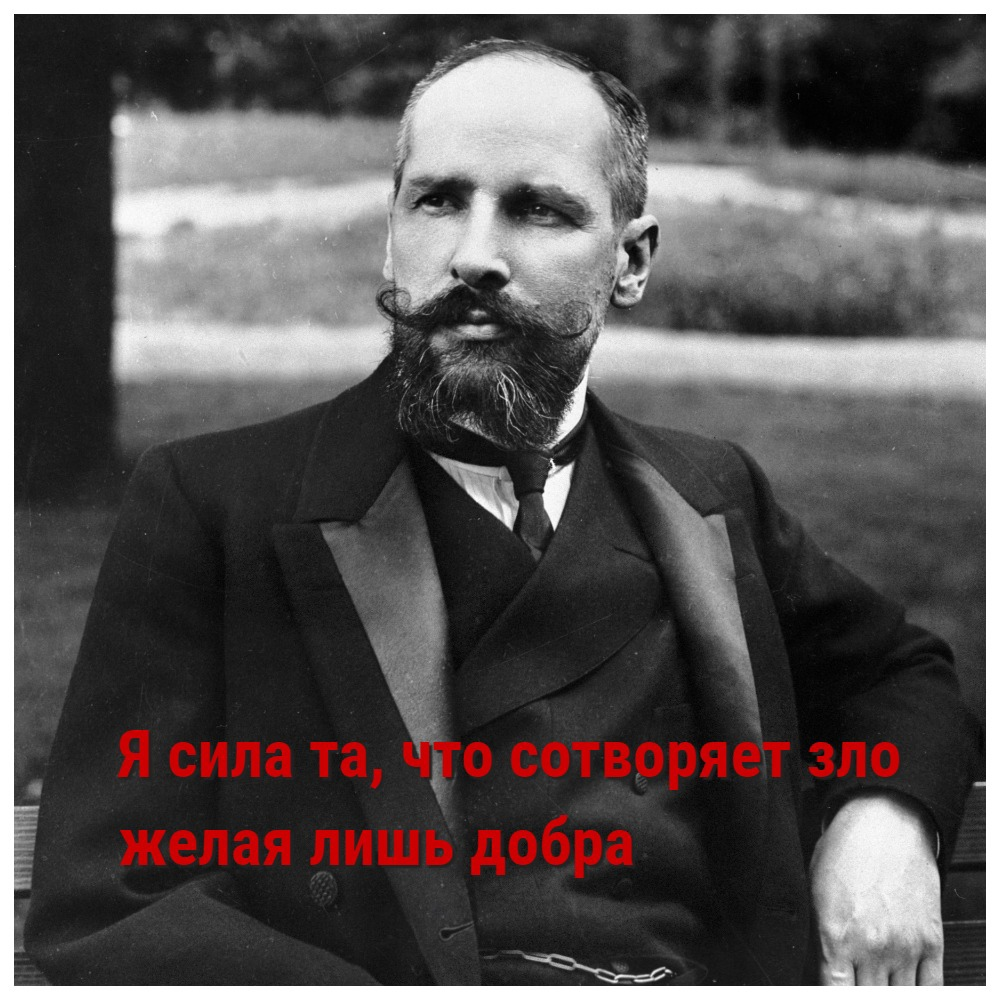
\includegraphics[scale=0.5]{Stolypin/UMLzLy9tOI4.jpg}
	%	\label{fig:scipion} % Unique label used for referencing the figure in-text\end{document}
	%	%\addcontentsline{toc}{figure}{Figure \ref{fig:placeholder}} % Uncomment to add the figure to the table of contents%----------------------------------------------------------------------------------------
	%\caption{Если искать в интернете инфу про отца Морлиона, то найдется очень много различной литературы про знаменитых шпионов. Так или иначе, за Морлионом закрепилось звание агента ЦРУ — что, судя по найденной мною инфе, неудивительно. Я не очень в шпионских делах - может, когда-нибудь... }%	CHAPTER 2
\end{figure}

Как все мы знаем ещё со школьной скамьи, Россия тогда была страной аграрной и, соответственно, вопрос № 1 всегда и везде это земля. Освобождение крестьян пусть и решило часть вопросов, способствовало росту промышленности и так далее, но, по большому счету, в далеком 1861 году была заложена огромная пороховая бочка и фитилёк к ней уже начинал гореть. И вот Николай II решает, что нужно прямо таки срочно кому-то заняться этим вопросом и назначает крайним нашего дорогого Петра Аркадьевича. Выбор был не случайным, после своих речей в думе, Столыпин зарекомендовал себя как монархиста, государственника и просто честного и неподкупного человека, короче говоря, он реально выделялся на фоне остальных чиновников того времени.

Я не буду пытаться утомить вас графиками и цифрами статистики, поясняющими почему же земельная реформа провалилась, а просто скромно улыбаясь, скажу, что таки да, “она утонула”. Утонула, прежде всего, в насилии и столь знакомой нам чиновничьей показухе. Взяв за образец прусский «хуторной» подход к развитию крестьянства, Столыпин как-то совершенно упустил из виду, что в Пруссии переход от общины к индивидуализму занял больше ста лет! Русский народ, конечно, славится своей способностью к форсированному переходу от одной экономической формации к другой, но простите… даже пятилетка в четыре года звучит разумнее.

Была проблема и с тем, что многие губернаторы, соревнуясь у кого лучше получается, заставляли крестьян выделяться из общины всеми правдами и неправдами, угрожая силой и канцелярской анафемой. А поскольку выход даже одного крестьянина из общины влечет передел земли у всех, вы можете сами себе представить, как это всем «нравилось», и так было по всей империи.

Такой подход не мог благотворно повлиять на протекание реформы. Столыпин задумывал создание целого слоя крепких хозяйственников – опору царского режима, а получил развал института крестьянской общины, усиление помещиков и исход бедняков в города, так что большевики говорят Столыпину большое спасибо за увеличение революционно настроенных маргиналов.

Столыпин хотел принести успокоение, но принес лишь новое всеобщее озлобление и ускорение революционных процессов. Неудачная реформа показала народу, что власть более не способна решать злободневные вопросы. Сложилась та ситуация, при которой верхи не могут править по-старому, а народ больше не желает их правления. Своими действиями Столыпин не потушил фитиль революции, а смачно так на него дунул. Хоть он и был, как личность в целом, неплохим человеком и желал для своей родины только хорошего, его попытка усидеть на двух стульях обернулась падением в бездну как для самого Столыпина, так и для империи.

А вопрос “можно ли было по-другому, можно ли было уберечь Россию от великих потрясений” – это, пожалуй, тема для отдельного и очень-очень большого лонга.

Автор Евгений Ляхович Ссылка \url{https://vk.com/wall-162479647_207869}
\#Ляхович@catx2
\#Заметка@catx2
